% !TeX program = pdflatex
% Source: dathuynh1108/OCC at 91223d63adc3289786bbdeff16d5feeb59aeb3d7.
% Same measured v2 snapshot. Added original-method sources, exact PatchCore feature path, Git links and rerun handoff. No new benchmark run.
\documentclass[aspectratio=169,professionalfonts,10pt]{beamer}
\usetheme{Boadilla}
\usecolortheme{default}
\setbeamertemplate{navigation symbols}{}
\usepackage[utf8]{inputenc}
\usepackage[T1]{fontenc}
\usepackage{lmodern}
\usepackage{amsmath,amssymb,amsfonts,mathtools,bm}
\usepackage{booktabs,array,tabularx,ragged2e}
\usepackage{graphicx,xcolor,tikz,etoolbox}
\usetikzlibrary{positioning,arrows.meta,calc}
\usepackage{hyperref}
\graphicspath{{assets/}}
\definecolor{navy}{RGB}{16,44,84}
\definecolor{teal}{RGB}{0,122,122}
\definecolor{orange}{RGB}{168,95,18}
\definecolor{softblue}{RGB}{233,240,250}
\definecolor{softgreen}{RGB}{232,244,239}
\definecolor{softorange}{RGB}{252,239,226}
\definecolor{softgray}{RGB}{245,245,245}
\setbeamercolor{title}{fg=navy}
\setbeamercolor{frametitle}{fg=navy,bg=navy!6}
\setbeamercolor{structure}{fg=navy}
\setbeamercolor{normal text}{fg=black,bg=white}
\setbeamercolor{block title}{fg=white,bg=navy}
\setbeamercolor{block body}{fg=black,bg=navy!5}
\setbeamercolor{block title alerted}{fg=orange,bg=softorange}
\setbeamercolor{block body alerted}{fg=black,bg=softorange!55}
\setbeamercolor{alerted text}{fg=orange}
\setbeamertemplate{blocks}[rounded][shadow=false]
\setbeamerfont{title}{series=\bfseries,size=\LARGE}
\setbeamerfont{frametitle}{series=\bfseries,size=\large}
\setbeamerfont{block title}{series=\bfseries,size=\normalsize}
\setbeamersize{text margin left=0.62cm,text margin right=0.62cm}
\def\phase{NBD}
\setbeamertemplate{footline}{%
\leavevmode\hbox to \paperwidth{\hspace{0.62cm}{\scriptsize\color{navy!65}\phase}\hfill
{\scriptsize\color{navy}\insertframenumber\,/\,\inserttotalframenumber}\hspace{0.6cm}}\vspace{0.13cm}}
\newcommand{\RR}{\mathbb R}
\newcommand{\MM}{\mathcal M}
\newcommand{\Cand}{\mathcal C}
\newcommand{\TT}{\mathcal T}
\newcommand{\norm}[1]{\left\lVert#1\right\rVert}
\newcommand{\head}[1]{\par{\normalsize\bfseries\color{navy}#1}\par\vspace{2pt}}
\newcommand{\remarktext}[1]{\par\smallskip{\footnotesize\color{navy!85}#1}\par}
\newcommand{\src}[1]{\par\smallskip{\scriptsize\color{navy!65}#1}\par}
\newcommand{\band}[1]{\begin{beamercolorbox}[rounded=true,sep=0.17cm]{block body}#1\end{beamercolorbox}}
\newcommand{\tightmath}{\setlength{\abovedisplayskip}{4pt}\setlength{\belowdisplayskip}{4pt}\setlength{\abovedisplayshortskip}{2pt}\setlength{\belowdisplayshortskip}{2pt}}
\appto\normalsize{\tightmath}\appto\small{\tightmath}\appto\footnotesize{\tightmath}
\newcolumntype{Y}{>{\RaggedRight\arraybackslash}X}
\title{Normality Bubble Diffusion}
\subtitle{Full MVTec AD results and model review}
\author{Huynh Thanh Dat}
\date{September 2026}
\hypersetup{pdftitle={Normality Bubble Diffusion},pdfauthor={Huynh Thanh Dat},pdfsubject={Full MVTec AD; shared frozen CNN benchmark; repo 91223d6}}

\newcommand{\resultsrc}[1]{\src{\href{https://github.com/dathuynh1108/OCC/tree/91223d63adc3289786bbdeff16d5feeb59aeb3d7/results/mvtec-full-v2}{OCC / mvtec-full-v2 @ 91223d6} \;|\; #1}}

\begin{document}

\def\phase{NBD}
\begin{frame}[plain]
\vspace{0.20cm}
\begin{center}
\begin{beamercolorbox}[wd=0.94\paperwidth,rounded=true,sep=0.38cm,center]{block title}
{\usebeamerfont{title}\color{white}Normality Bubble Diffusion}\\[0.3em]
{\large\color{white}Full MVTec AD results and model review}
\end{beamercolorbox}
\vspace{0.18cm}
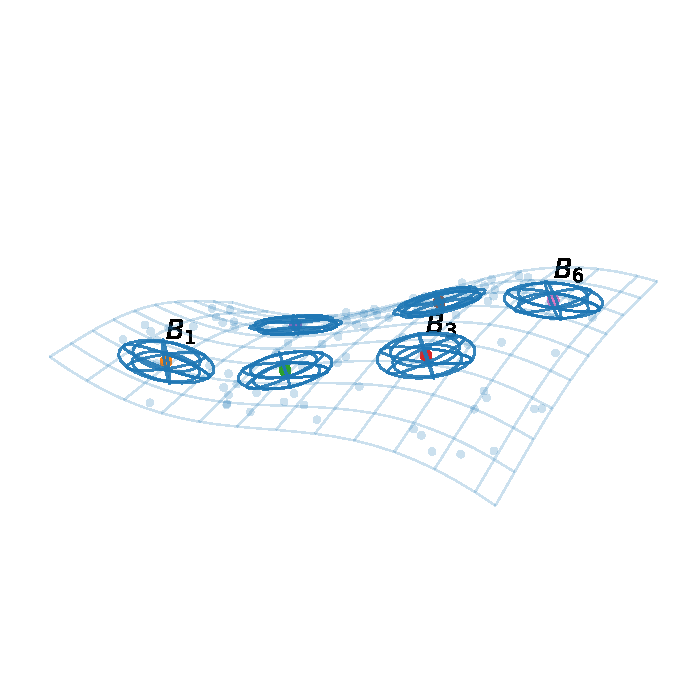
\includegraphics[width=10.1cm,height=3.5cm,keepaspectratio]{manifold3d.pdf}
\par\vspace{0.06cm}
{\large\textbf{Huynh Thanh Dat}}\quad{\normalsize 14 September 2026}
\vspace{0.28cm}
\par{\small Baselines $\;\to\;$ Baseline results $\;\to\;$ NBD $\;\to\;$ Comparison}
\end{center}
\end{frame}

\def\phase{PROBLEM}
\begin{frame}[t]{One-class detection}
\vspace{0.23cm}
\begin{columns}[T,onlytextwidth]
\column{.40\textwidth}
\head{Train on normal data}
\[
\mathcal D_N=\{x_i\}_{i=1}^{n}.
\]
\vspace{0.15cm}
\head{Score new observations}
\[
s(x):\mathcal X\to\RR.
\]
A larger score means more anomalous.
\vspace{0.30cm}
\band{Training and calibration: normal only.\\[0.1cm]Test: normal + anomaly.}
\column{.56\textwidth}
\centering
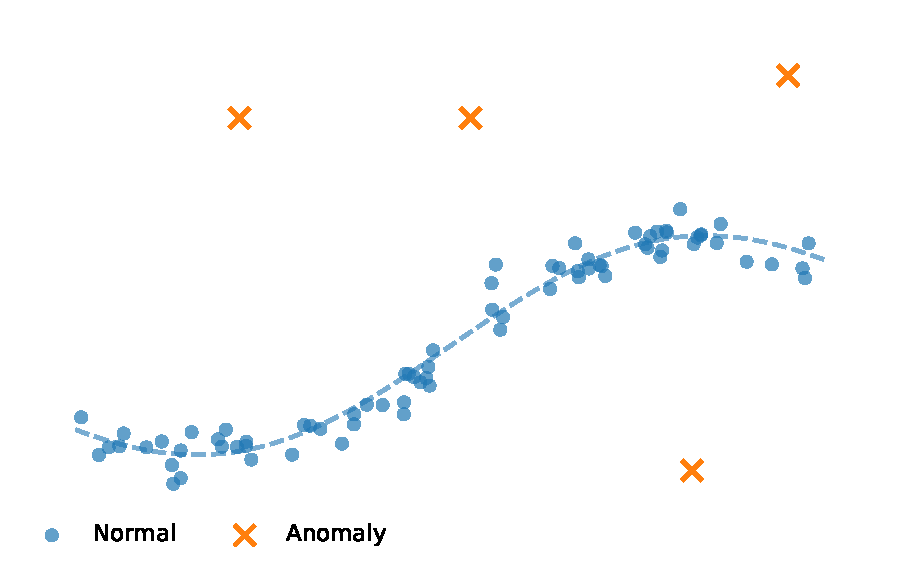
\includegraphics[width=\linewidth,height=4.8cm,keepaspectratio]{problem.pdf}
\src{Schematic: normal support can be curved.}
\end{columns}
\vspace{0.28cm}
\remarktext{Image benchmark: $z_p=f_{\rm CNN}(x)_p$; the same frozen CNN descriptors are used by every method.}
\end{frame}


\def\phase{PAPER SOURCES}
\begin{frame}[t]{The original methods do not share one backbone}
\small
\vspace{.08cm}
\begin{columns}[T,onlytextwidth]
\column{.48\textwidth}
\begin{block}{PatchCore --- Roth et al.}
\textbf{ImageNet-pretrained Wide ResNet-50.}\\[.06cm]
Freeze the CNN; extract intermediate patches.\\
Build a normal-feature memory, not a learned head.
\par\vspace{.10cm}
\href{https://github.com/amazon-science/patchcore-inspection/tree/fcaa92f124fb1ad74a7acf56726decd4b27cbcad}{\textcolor{teal}{GitHub: amazon-science/patchcore-inspection}}
\end{block}
\begin{block}{SVDD --- Tax and Duin}
\textbf{No CNN in the original method.}\\[.06cm]
A kernel maps the chosen input features.\\
A quadratic program fits the enclosing sphere.
\par\vspace{.10cm}
\href{https://github.com/DMJTax/dd_tools/tree/efaaf04efae1f8be78906836a5d31547b48be7af}{\textcolor{teal}{GitHub: DMJTax/dd\_tools (author toolbox)}}
\end{block}
\column{.48\textwidth}
\begin{block}{Deep SVDD --- Ruff et al.}
\textbf{Trainable LeNet-type image CNN.}\\[.06cm]
Initialize from a normal-image autoencoder;\\
then optimize the encoder with the SVDD loss.
\par\vspace{.10cm}
\href{https://github.com/lukasruff/Deep-SVDD/tree/e20f18c8d0ad9dc01cad09fdf311bd861351a9ad}{\textcolor{teal}{GitHub: lukasruff/Deep-SVDD (paper code)}}
\end{block}
\begin{block}{DROCC --- Goyal et al.}
\textbf{Trainable LeNet on CIFAR-10.}\\[.06cm]
Search for negatives in the image input space.\\
ImageNet-10 uses a different CNN: MobileNetV2.
\par\vspace{.10cm}
\href{https://github.com/microsoft/EdgeML/tree/81025fce8ba28707eabe72e11bf3987a8d745608/examples/pytorch/DROCC}{\textcolor{teal}{GitHub: microsoft/EdgeML / DROCC}}
\end{block}
\end{columns}
\vspace{.08cm}
\band{\footnotesize \textbf{PatchScore} is our project baseline. The source paper is \textbf{PatchCore}.\\[.04cm]
The existing MVTec tables below compare shared-CNN adaptations, not native-paper reproductions.}
\end{frame}

\def\phase{AUTHOR CODE}
\begin{frame}[t]{PatchCore: author feature extractor}
\small
\remarktext{Author Quick Guide: ImageNet-pretrained WRN-50 / 224 input / 1,024-D / 10\% coreset.}
\vspace{.12cm}
\begin{center}
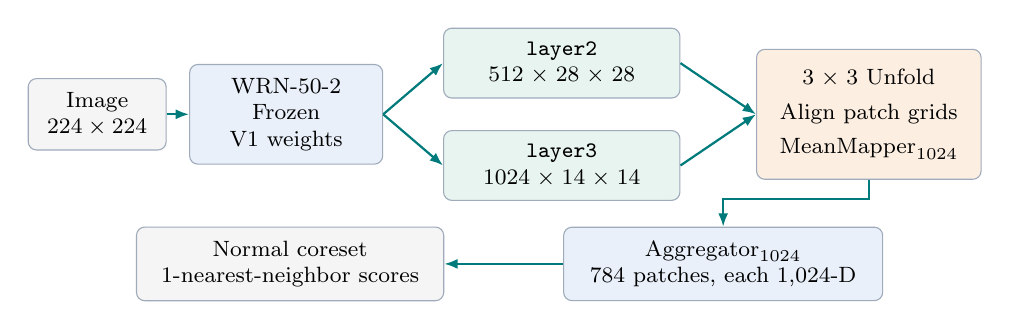
\begin{tikzpicture}[
 box/.style={rounded corners=3pt,draw=navy!40,minimum height=.88cm,align=center,inner sep=5pt,font=\footnotesize},
 arr/.style={-{Latex[length=1.7mm]},thick,draw=teal}]
\node[box,fill=softgray,text width=1.40cm] (im) at (0,0) {Image\\$224\times224$};
\node[box,fill=softblue,text width=2.10cm] (cnn) at (2.4,0) {WRN-50-2\\Frozen\\V1 weights};
\node[box,fill=softgreen,text width=2.65cm] (l2) at (5.9,.65) {\texttt{layer2}\\$512\times28\times28$};
\node[box,fill=softgreen,text width=2.65cm] (l3) at (5.9,-.65) {\texttt{layer3}\\$1024\times14\times14$};
\node[box,fill=softorange,text width=2.50cm,minimum height=1.65cm] (patch) at (9.8,0) {$3\times3$ Unfold\\\smallskip Align patch grids\\\smallskip $\operatorname{MeanMapper}_{1024}$};
\draw[arr](im)--(cnn);\draw[arr](cnn.east)--(l2.west);\draw[arr](cnn.east)--(l3.west);
\draw[arr](l2.east)--(patch.west);\draw[arr](l3.east)--(patch.west);
\node[box,fill=softblue,text width=3.7cm] (agg) at (7.95,-1.90) {$\operatorname{Aggregator}_{1024}$\\784 patches, each 1,024-D};
\node[box,fill=softgray,text width=3.55cm] (mem) at (2.45,-1.90) {Normal coreset\\1-nearest-neighbor scores};
\draw[arr](patch.south)--++(0,-.24)-|(agg.north);\draw[arr](agg.west)--(mem.east);
\end{tikzpicture}
\end{center}
\vspace{-.10cm}
\band{\footnotesize \textbf{Our recorded v2 run:} spatial averaging + concatenation gives \textbf{1,536-D}, not the author-code 1,024-D descriptor. Its top-1\% mean is also different from the author-code image maximum.}
\src{Paper Eq. (7): extra neighbor reweighting. Inspected author code: maximum patch score. Separate targets.}
\src{\href{https://github.com/amazon-science/patchcore-inspection/blob/fcaa92f124fb1ad74a7acf56726decd4b27cbcad/src/patchcore/patchcore.py}{\textcolor{teal}{GitHub: patchcore.py}}\quad
\href{https://github.com/amazon-science/patchcore-inspection/blob/fcaa92f124fb1ad74a7acf56726decd4b27cbcad/src/patchcore/common.py}{\textcolor{teal}{common.py}}\quad
\href{https://github.com/amazon-science/patchcore-inspection/blob/fcaa92f124fb1ad74a7acf56726decd4b27cbcad/README.md}{\textcolor{teal}{Author run command}}}
\end{frame}

\def\phase{METHODS}
\begin{frame}[t]{PatchScore: the recorded shared-CNN baseline}
\small
\begin{columns}[T,onlytextwidth]
\column{.49\textwidth}
\centering
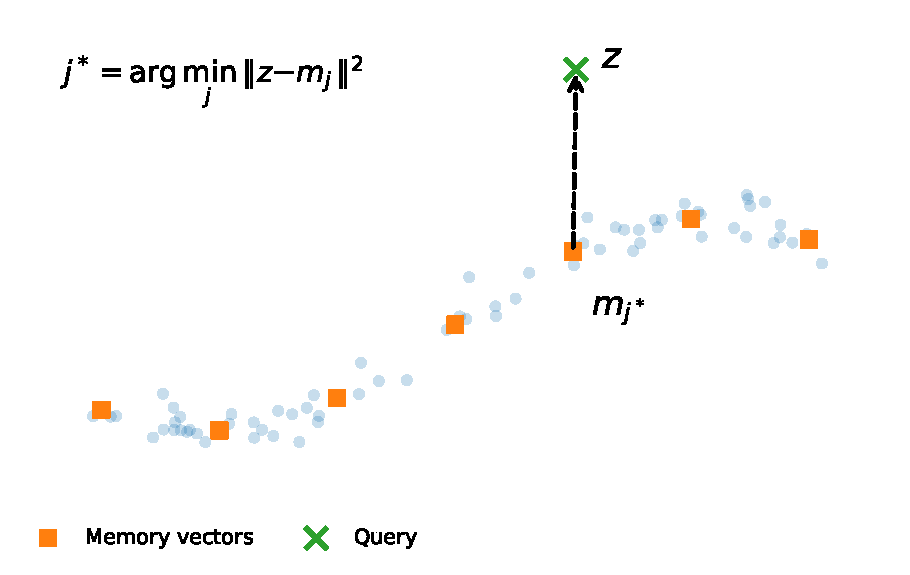
\includegraphics[width=\linewidth,height=2.60cm,keepaspectratio]{patchscore.pdf}
\par\vspace{0.10cm}
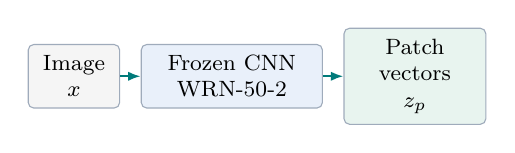
\begin{tikzpicture}[
box/.style={rounded corners=2pt,draw=navy!40,align=center,inner sep=4pt,
minimum height=.80cm,font=\footnotesize},
arr/.style={-{Latex[length=1.6mm]},thick,draw=teal}]
\node[box,fill=softgray,text width=.88cm] (x) {Image\\$x$};
\node[box,fill=softblue,text width=2.02cm,right=.26cm of x] (f) {Frozen CNN\\WRN-50-2};
\node[box,fill=softgreen,text width=1.52cm,right=.26cm of f] (z) {Patch vectors\\$z_p$};
\draw[arr](x)--(f);\draw[arr](f)--(z);
\end{tikzpicture}
\par\vspace{.15cm}
\[
s_{\rm PS}(z)=\min_{m_j\in\mathcal M}\norm{z-m_j}_2^2.
\]
\column{.47\textwidth}
\head{Backbone used in this benchmark}
\textbf{Wide ResNet-50-2}, frozen/eval.\\
ImageNet-1K V1; \texttt{layer2 + layer3}.\\[.10cm]
Resize 256; center crop 224.\\
Local $3\times3$ averaging, bilinear alignment.\\
$28\times28$ patches; 1,536-D each. No global PCA.
\vspace{.18cm}
\head{Memory for the baseline comparison}
\textbf{128 normal centers.} Select farthest-first anchors from fit patches; take the mean of each anchor's 128-neighbor set.\\[.12cm]
Score a query by its nearest center. A larger-memory control is compared later.
\end{columns}
\vspace{.06cm}
\band{\small All methods use the \textbf{mean of the top 1\% patch scores} for each image.}
\vfill
\resultsrc{Historical v2: \texttt{configs/full.json}. Reference: \href{https://github.com/amazon-science/patchcore-inspection}{\textcolor{teal}{PatchCore GitHub}}. Not the author-code pipeline.}
\end{frame}

\def\phase{METHODS}
\begin{frame}[t]{SVDD and Deep SVDD on frozen CNN features}
\vspace{0.05cm}
\begin{columns}[T,onlytextwidth]
\column{.48\textwidth}
\head{RBF SVDD}
\centering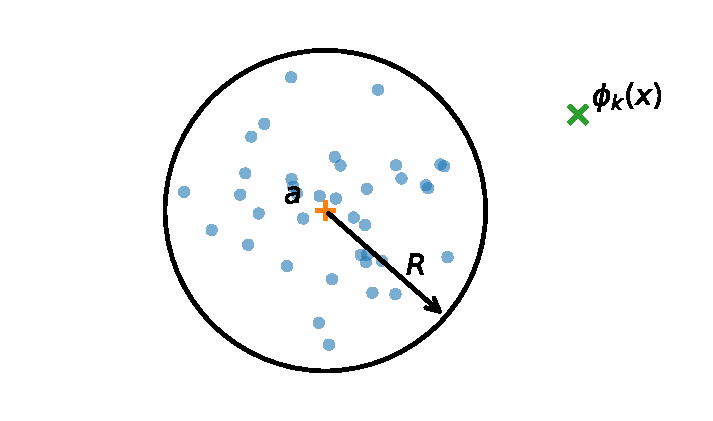
\includegraphics[width=.92\linewidth,height=2.30cm,keepaspectratio]{svdd.pdf}\par
\raggedright\small
\[
\min_{a,R,\xi\ge0} R^2+C\sum_i\xi_i,
\]
\[
\text{s.t. }\norm{\phi_k(z_i)-a}^2\le R^2+\xi_i.
\]
\[
s_{\rm SVDD}(z)=\norm{\phi_k(z)-a}^2-R^2.
\]
\remarktext{Dual QP on 2,048 normal coreset patches.\\$\nu=0.1$; bandwidth from median pair distance.}
\column{.48\textwidth}
\head{Deep SVDD-head}
\centering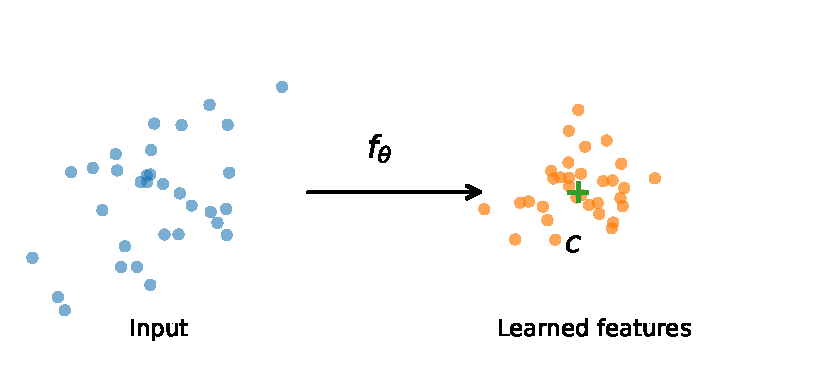
\includegraphics[width=.99\linewidth,height=2.30cm,keepaspectratio]{deep_svdd.pdf}\par
\raggedright\small
\[
\min_\theta\frac1n\sum_i\norm{g_\theta(z_i)-c}^2
+\frac\lambda2\norm\theta^2.
\]
\[
s_{\rm DSVDD}(z)=\norm{g_\theta(z)-c}^2.
\]
\vspace{0.04cm}
\remarktext{Bias-free $1536\to64\to16$ head; fixed $c\ne0$.\\50 AE + 100 SVDD epochs; all fit patches.}
\end{columns}
\vspace{0.2cm}
\src{Author sources: \href{https://github.com/DMJTax/dd_tools}{\textcolor{teal}{SVDD GitHub}}\quad
\href{https://github.com/lukasruff/Deep-SVDD}{\textcolor{teal}{Deep SVDD paper-code GitHub}}\quad
\href{https://github.com/lukasruff/Deep-SVDD-PyTorch}{\textcolor{teal}{Author PyTorch GitHub}}.}
\resultsrc{Recorded adaptation: capped kernel support; the Deep SVDD head does not fine-tune the CNN.}
\end{frame}

\def\phase{METHODS}
\begin{frame}[t]{Deep SVDD: collapse and safeguards}
\small
\remarktext{Shared-CNN setup: $z$ is a frozen descriptor; only $g_\theta$ is trained.}
\vspace{0.10cm}
\begin{columns}[T,onlytextwidth]
\column{.47\textwidth}
\head{Collapse $\ne$ compactness}
Normal compactness is intended. A constant mapping loses all input information.
\begin{alertblock}{Trivial mapping}
\[
 g_\theta(z)\equiv c\quad\Longrightarrow\quad s(z)=0.
\]
\small Normal and anomalous queries get the same score.
\end{alertblock}
\vspace{0.08cm}
A bias provides an easy constant-map solution:
\[
 g_\theta(z)=Wh(z)+b,\quad W=0,\ b=c.
\]
\remarktext{Only the data term is necessarily zero.}
\column{.49\textwidth}
\head{Controls in the current code}
\textbf{No bias.} Both trainable head layers use
\texttt{bias=False}.
\par\vspace{0.14cm}
\textbf{Fixed nonzero center.} Compute $c$ once from normal outputs; do not optimize it.
\par\vspace{0.14cm}
\textbf{ReLU.} Avoid bounded activations with nonzero saturation.
\par\vspace{0.14cm}
\textbf{AE pretraining.} Reconstruct normal features, then discard the decoder before SVDD.
\end{columns}
\vspace{0.12cm}
\band{\footnotesize AE gives an initialization, not a guarantee against collapse.
The code logs final output variance as a diagnostic.}
\vfill
\src{Ruff et al., Sec. 3.3. \href{https://github.com/lukasruff/Deep-SVDD}{\textcolor{teal}{Paper-code GitHub}}. Controls shown here refer to the recorded shared-feature head.}
\end{frame}

\def\phase{METHODS}
\begin{frame}[t]{DROCC-head: negatives in CNN feature space}
\small
\begin{block}{Normal label: 1 \hspace{0.4cm} Generated label: 0}
\[
\min_\theta\frac1n\sum_i\left[\ell(g_\theta(z_i),1)
+\mu\max_{r\le\norm{h}_2\le\gamma r}\ell(g_\theta(z_i+h),0)\right]
+\frac\lambda2\norm\theta^2.
\]
\end{block}
\vspace{0.05cm}
\begin{columns}[T,onlytextwidth]
\column{.43\textwidth}
\centering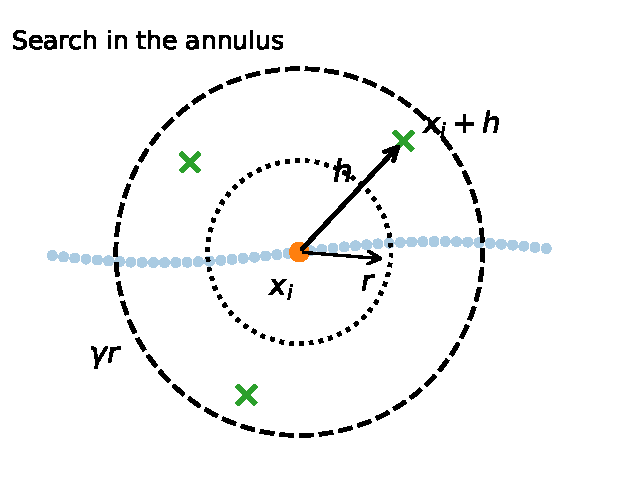
\includegraphics[width=\linewidth,height=3.12cm,keepaspectratio]{drocc.pdf}
\column{.53\textwidth}
\head{Training}
Warm up on normal data.\\[0.08cm]
Ascend in $h$; project back to the annulus.\\[0.08cm]
Update $\theta$ to separate the two labels.
\vspace{0.05cm}
\head{Settings used}
$1536\to64\to1$ MLP; 100 epochs (10 warm-up).\\
50 ascent steps; $\gamma=2$, $\mu=1$.\\
$r=0.5\times$ median normal 5-NN distance.\\
Ascent step $0.05r$; score $s(z)=-g_\theta(z)$.
\end{columns}
\src{Native reference: \href{https://github.com/microsoft/EdgeML/tree/81025fce8ba28707eabe72e11bf3987a8d745608/examples/pytorch/DROCC}{\textcolor{teal}{microsoft/EdgeML / DROCC (GitHub)}}.}
\resultsrc{Recorded feature-space adaptation, not original image DROCC. Batch 8,192; all fit patches per epoch.}
\end{frame}

\def\phase{SHARED SETUP}
\begin{frame}[t]{MVTec AD: shared evaluation setup}
\small
\vspace{.10cm}
\begin{center}
\renewcommand{\arraystretch}{1.30}
\begin{tabular}{lrrr}
\toprule
&\textbf{Train normal}&\textbf{Test normal}&\textbf{Test anomaly}\\
\midrule
All 15 categories&3,629&467&1,258\\
\bottomrule
\end{tabular}
\end{center}
\vspace{.12cm}
\begin{center}
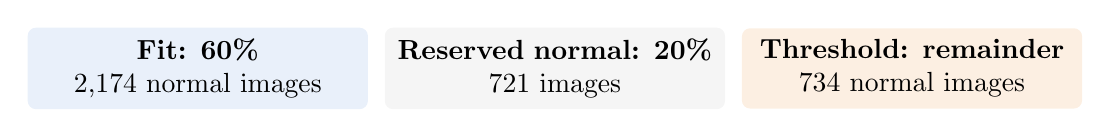
\begin{tikzpicture}[box/.style={rounded corners=3pt,minimum height=1.02cm,text width=4.04cm,align=center,inner sep=4pt}]
\node[box,fill=softblue] (fit) {\textbf{Fit: 60\%}\\2,174 normal images};
\node[box,fill=softgray,right=.20cm of fit] (reserved) {\textbf{Reserved normal: 20\%}\\721 images};
\node[box,fill=softorange,right=.20cm of reserved] (thr) {\textbf{Threshold: remainder}\\734 normal images};
\end{tikzpicture}
\end{center}
\remarktext{Per-seed totals across categories. Split by image, before extracting patches.}
\vspace{.08cm}
\textbf{Reserved images are unused by these four baselines.} Fit on the left subset; set image thresholds on the right subset.
\par\vspace{.18cm}
Same frozen CNN descriptors and splits; seeds \textbf{0, 1, 2}. All test images retained.\\[.08cm]
Models and thresholds are fixed before testing.
\vspace{.13cm}
\band{\small Metrics: image AUROC / AP and FPR / TPR. Image score: mean of the top 1\% patches.}
\vfill
\resultsrc{\texttt{REPORT.md}, \texttt{configs/full.json}. Shared-feature comparison; not the original paper benchmarks.}
\end{frame}

\def\phase{BASELINE RESULTS}
\begin{frame}[t]{Baseline results on MVTec AD}
\centering
\vspace{.08cm}
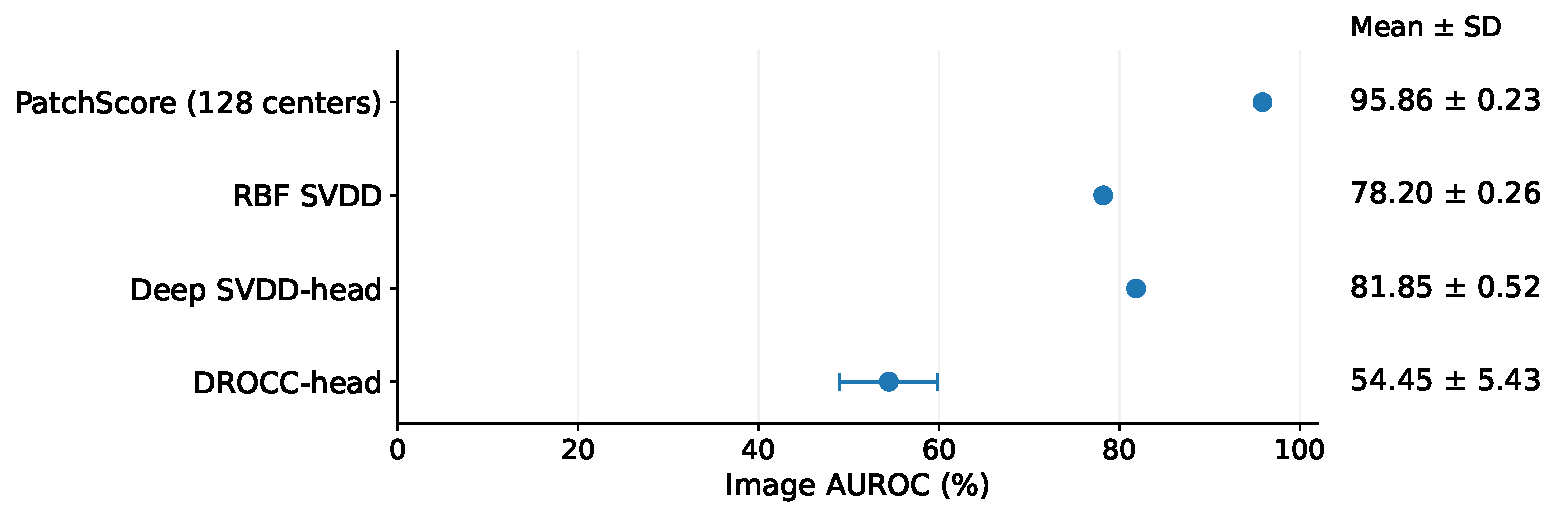
\includegraphics[width=.97\textwidth,height=4.15cm,keepaspectratio]{mvtec_baseline_auroc.pdf}
\par\vspace{.13cm}
\band{\small PatchScore with 128 centers has the highest image AUROC among these four baselines.}
\raggedright
\remarktext{Mean $\pm$ sample SD of three seed means. Each seed averages the 15 categories equally.}
\resultsrc{\texttt{summary.csv}. PatchScore (128 centers) is the published \texttt{PatchScore\_same\_centers} row.}
\end{frame}

\def\phase{BASELINE RESULTS}
\begin{frame}[t]{Image thresholds and baseline operating points}
\small
\begin{columns}[T,onlytextwidth]
\column{.49\textwidth}
\head{One threshold per method, category and seed}
Sort the $n$ image scores in the normal threshold subset:
\[
k=\left\lceil(n+1)(1-\alpha)\right\rceil,\qquad\alpha=0.05,
\]
\[
\tau=\begin{cases}s_{(k)},&k\le n,\\+\infty,&k>n,\end{cases}
\qquad\widehat y=\mathbf1\{s(x)>\tau\}.
\]
\vspace{.12cm}
No fit images or test labels are used to estimate $\tau$.
\vspace{.22cm}
\band{\footnotesize \textbf{Toothbrush:} $n=12$, so $k=13$ and $\tau=+\infty$. Its zero FPR/TPR is retained.}
\column{.47\textwidth}
\head{Measured test FPR and TPR (\%)}
\footnotesize
\renewcommand{\arraystretch}{1.48}\setlength{\tabcolsep}{4pt}
\begin{tabular}{lrr}
\toprule
\textbf{Method}&\textbf{FPR}&\textbf{TPR}\\
\midrule
PatchScore (128 centers) & 11.36 & 79.28 \\
RBF SVDD & 6.86 & 45.26 \\
Deep SVDD-head & 6.88 & 49.56 \\
DROCC-head & 3.51 & 8.38 \\
\bottomrule
\end{tabular}
\vspace{.22cm}
\remarktext{Macro averages over categories and seeds. AUROC measures ranking; this table uses the fixed thresholds.}
\end{columns}
\vfill
\band{\small $\alpha=5\%$ is a calibration target, \textbf{not} the observed test FPR.}
\resultsrc{\texttt{summary.csv}, reported threshold protocol. These image-threshold rules are shared by all methods.}
\end{frame}

\def\phase{BASELINE DIAGNOSTICS}
\begin{frame}[t]{Training diagnostics: Deep SVDD and DROCC}
\small
\vspace{.12cm}
\begin{columns}[T,onlytextwidth]
\column{.48\textwidth}
\head{Deep SVDD-head}
Image AUROC: \textbf{81.85 $\pm$ 0.52\%}.
\begin{block}{Output variance ratio}
\[
\frac{\text{final normal output variance}}{\text{initial normal output variance}}
\]
\small Median: \textbf{0.0009754}.\\[.08cm]
Range: $0.0001308$--$0.0116951$ over 45 runs.
\end{block}
\remarktext{Strong contraction. This alone does not establish a constant mapping or an implementation error.}
\column{.48\textwidth}
\head{DROCC-head}
Image AUROC: \textbf{54.45 $\pm$ 5.43\%}.
\begin{block}{Final training loss}
\small Median: \textbf{1.3862944} over 45 runs.\\[.18cm]
Measured test TPR: \textbf{8.38\%}.
\end{block}
\remarktext{Weak detection in this shared-feature adaptation. This is not the original DROCC paper's benchmark result.}
\end{columns}
\vspace{.20cm}
\band{\small Every fit patch was used in every epoch; batch size 8,192.\\[.08cm]
Terminal checkpoints were used regardless of their test performance.}
\vfill
\resultsrc{Reported training diagnostics; no training or checkpoint replay was repeated for this slide revision.}
\end{frame}

\def\phase{NBD MODEL}
\begin{frame}[t]{NBD: local bubbles, one shared graph}
\vspace{0.13cm}
\begin{columns}[T,onlytextwidth]
\column{.65\textwidth}
\centering
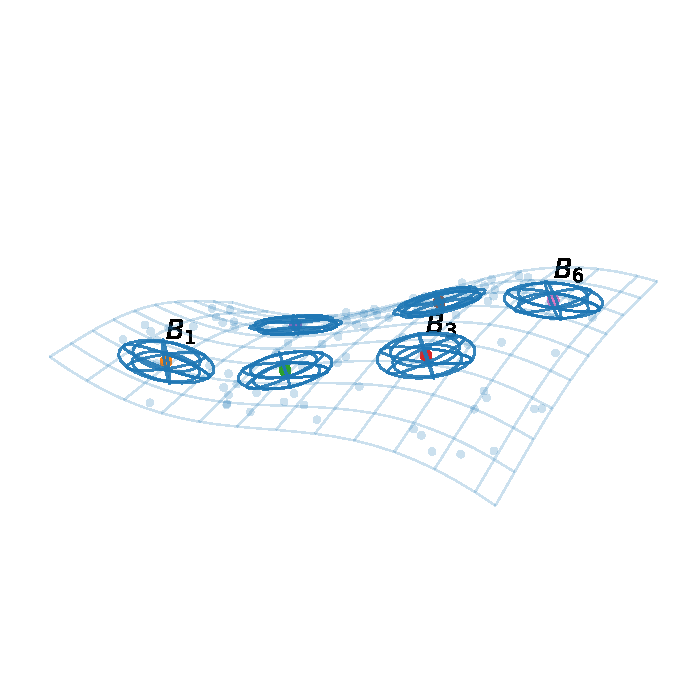
\includegraphics[width=\linewidth,height=4.2cm,keepaspectratio]{manifold3d.pdf}
\src{Schematic: local ellipsoids around a curved surface.}
\column{.31\textwidth}
\head{Each bubble stores}
A center, tangent variation, and normal thickness.
\vspace{0.34cm}
\head{The graph connects them}
Diffusion compares the regions each bubble can reach.
\end{columns}
\vspace{0.28cm}
\band{\centering Normal features $\to$ bubbles $\to$ shared graph $\to$ diffusion distance $\to$ query score}
\remarktext{Hypothesis tested: a normal query has local support and attaches to a coherent region of the graph.}
\end{frame}

\def\phase{NBD MODEL}
\begin{frame}[t]{A local normality bubble}
\small
\[
B_j=(c_j,U_j,\Lambda_j,\sigma_{\perp,j}^2),\qquad
U_j^\top U_j=I_{d_j},\qquad\Pi_j=U_jU_j^\top.
\]
\begin{columns}[T,onlytextwidth]
\column{.57\textwidth}
\head{Local model}
\[
z=c_j+U_ja+\varepsilon_{\perp,j},\qquad a\perp\!\!\!\perp\varepsilon_{\perp,j},
\]
\[
a\sim\mathcal N(0,\Lambda_j),\qquad
\varepsilon_{\perp,j}\sim\mathcal N\!\left(0,\sigma_{\perp,j}^2(I-\Pi_j)\right).
\]
\[
\boxed{\Sigma_j=U_j\Lambda_jU_j^\top+\sigma_{\perp,j}^2(I-\Pi_j).}
\]
\column{.39\textwidth}
\centering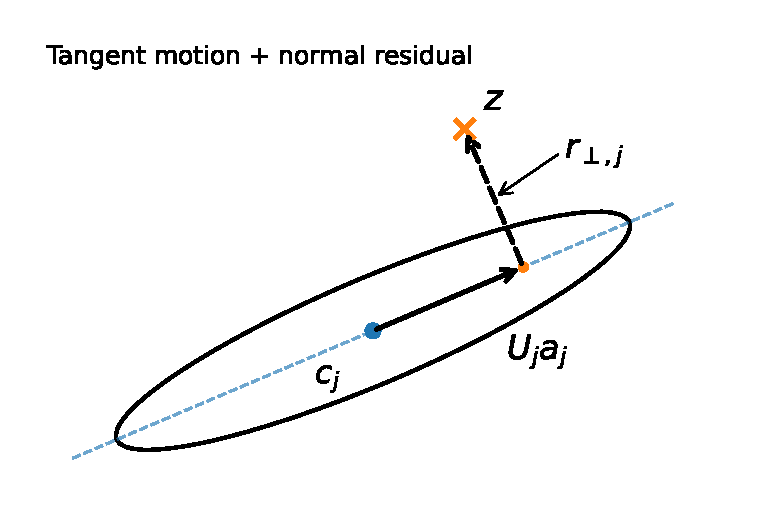
\includegraphics[width=\linewidth,height=2.90cm,keepaspectratio]{bubble_detail.pdf}
\end{columns}
\vspace{0.10cm}
\head{Fit by local PCA}
Neighborhood mean $\to c_j$; top $d_j$ eigenpairs $\to U_j,\Lambda_j$.
\[
\sigma_{\perp,j}^2=\frac1{D-d_j}\sum_{k=d_j+1}^{D}\widehat\lambda_{jk}.
\]
\remarktext{Executed: 128 bubbles; 128 neighbors; $d_j=16$. The same-center control uses the fitted neighborhood means $c_j$.}
\end{frame}

\def\phase{NBD MODEL}
\begin{frame}[t]{Scoring a query}
\small
\[
a_j(z)=U_j^\top(z-c_j),\qquad
r_{\perp,j}(z)=(I-\Pi_j)(z-c_j).
\]
\begin{block}{Local energy}
\[
E_j(z)=
\underbrace{\frac{a_j^\top(\Lambda_j+\epsilon I)^{-1}a_j}{d_j}}_{\text{tangent rarity}}
+\beta\underbrace{\frac{\norm{r_{\perp,j}}_2^2}{(D-d_j)(\sigma_{\perp,j}^2+\epsilon)}}_{\text{off-manifold residual}}.
\]
\end{block}
\vspace{0.02cm}
\begin{columns}[T,onlytextwidth]
\column{.48\textwidth}
\head{Absolute fit}
\[
S_B(z)=\min_{j\in\Cand(z)}E_j(z),
\]
\[
S_A(z)=-T_b\log\!\left[\frac1K\sum_{j\in\Cand(z)}e^{-E_j(z)/T_b}\right].
\]
\column{.48\textwidth}
\head{Attachment to the graph}
\[
b_j(z)=\frac{e^{-E_j(z)/T_b}}{\sum_{k\in\Cand(z)}e^{-E_k(z)/T_b}}.
\]
\remarktext{$K=|\Cand(z)|$ candidates; $b_j=0$ outside.\\$\sum_jb_j(z)=1$.}
\end{columns}
\src{Executed: $K=8$, $T_b=1$, $\beta=1$, $\epsilon=10^{-6}$. This dimension-normalized energy is not Gaussian NLL.}
\end{frame}

\def\phase{NBD MODEL}
\begin{frame}[t]{Comparing two bubbles}
\small
\vspace{0.08cm}
\begin{columns}[T,onlytextwidth]
\column{.322\textwidth}
\head{Center displacement}
\centering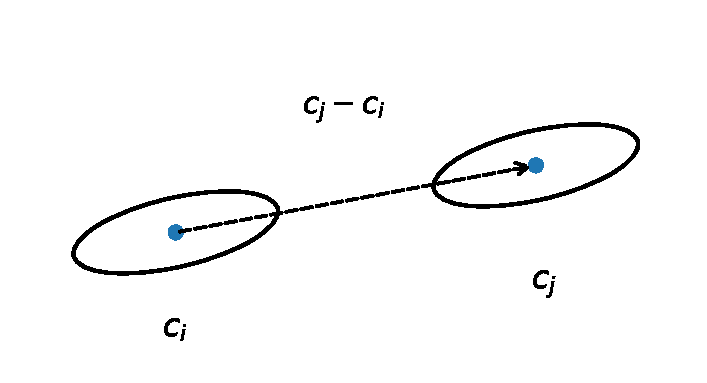
\includegraphics[width=\linewidth,height=1.68cm,keepaspectratio]{pair_centers.pdf}\par\raggedright
\remarktext{Earlier: Euclidean distance}
\[
r_c^{\rm E}(i,j)=\norm{c_i-c_j}_2^2.
\]
\remarktext{Used here: two-way bubble energy}
\[
r_c^{\rm G}(i,j)=\tfrac12\big[E_i(c_j)+E_j(c_i)\big].
\]
\column{.322\textwidth}
\head{Frame disagreement}
\centering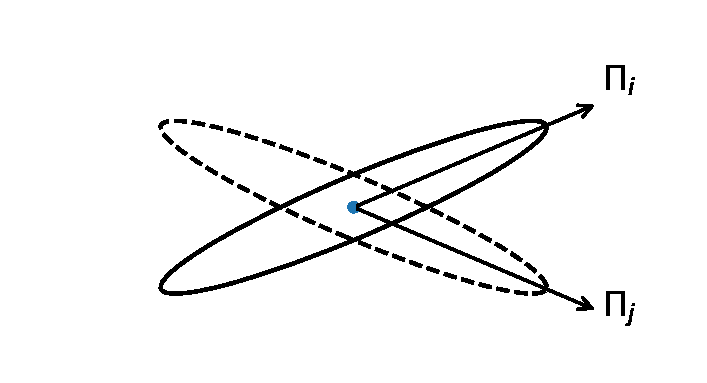
\includegraphics[width=\linewidth,height=1.68cm,keepaspectratio]{pair_frames.pdf}\par\raggedright
\[
r_F(i,j)=\norm{\Pi_i-\Pi_j}_F^2
\]
\[
=d_i+d_j-2\norm{U_i^\top U_j}_F^2.
\]
\remarktext{Compare tangent subspaces, not basis-vector signs.}
\column{.322\textwidth}
\head{Optional: thickness}
\centering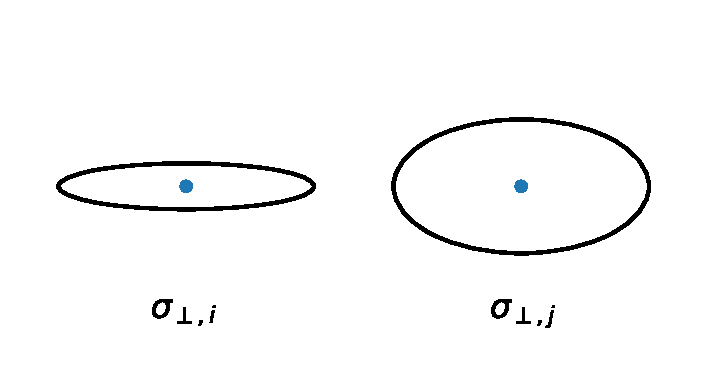
\includegraphics[width=\linewidth,height=1.68cm,keepaspectratio]{pair_thickness.pdf}\par\raggedright
\[
r_\sigma(i,j)=\left[\log\frac{\sigma_{\perp,i}^2+\epsilon}{\sigma_{\perp,j}^2+\epsilon}\right]^2.
\]
\remarktext{Not used in the reported benchmark. Not a full covariance distance.}
\end{columns}
\vspace{0.34cm}
\band{\textbf{Executed graph:} two-way center energy + frame disagreement. Thickness weight is zero.}
\src{The earlier Euclidean distance and the optional thickness term are shown for context, not as tested ablations.}
\end{frame}

\def\phase{NBD MODEL}
\begin{frame}[t]{From bubbles to a graph}
\small
\begin{block}{Edge dissimilarity, before diffusion}
\[
\delta_B(i,j)=\frac{r_c(i,j)}{\tau_c}
+\lambda_F\frac{r_F(i,j)}{\tau_F}.
\]
\end{block}
\begin{columns}[T,onlytextwidth]
\column{.49\textwidth}
\centering\vspace{.20cm}
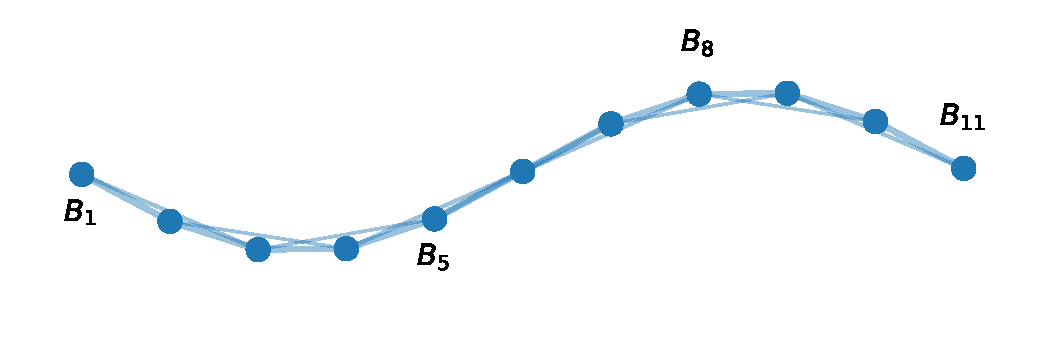
\includegraphics[width=\linewidth,height=2.85cm,keepaspectratio]{bubble_graph.pdf}
\src{Toy graph. Each node is one bubble; thicker edges have larger affinity.}
\column{.47\textwidth}
\head{Affinity and transition}
For symmetric local candidate edges $\mathcal E$,
\[
W_{ij}=\mathbf1_{\{(i,j)\in\mathcal E\}}e^{-\delta_B(i,j)}\quad(i\ne j),
\]
\[
W_{ii}=\eta>0,\qquad s_i=\sum_jW_{ij},
\]
\[
P_{ij}=\frac{W_{ij}}{s_i},\qquad\pi_i=\frac{s_i}{\sum_m s_m}.
\]
\end{columns}
\vspace{0.18cm}
\band{Fit the graph once on normal data. Every query uses the same bubble nodes.}
\src{Executed: 12 graph neighbors; $\lambda_F=1$, $\eta=1$. No thickness penalty. $\delta_B$ need not be a metric.}
\end{frame}

\def\phase{NBD MODEL}
\begin{frame}[t]{Diffusion distance}
\small
Similar $t$-step transition distributions give a smaller diffusion distance:
\[
\boxed{D_t^2(i,j)=\sum_m\frac{\big[(P^t)_{im}-(P^t)_{jm}\big]^2}{\pi_m}.}
\]
\begin{columns}[T,onlytextwidth]
\column{.44\textwidth}
\centering\vspace{0.12cm}
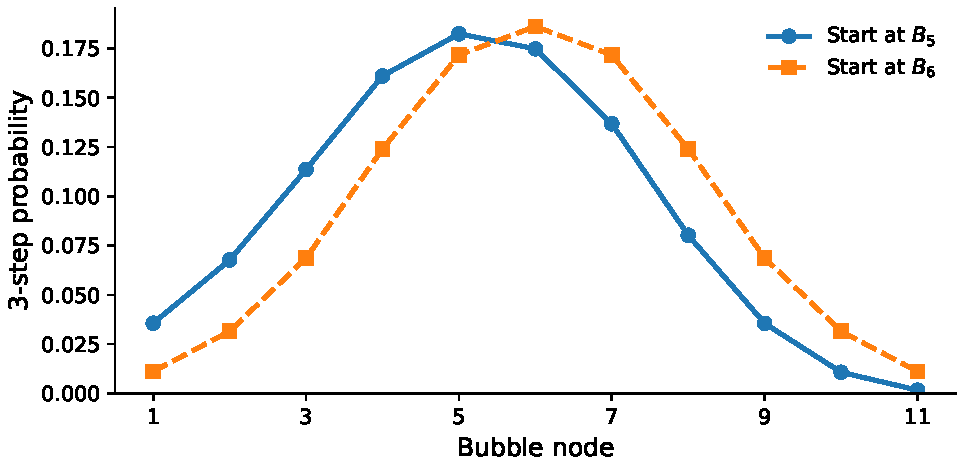
\includegraphics[width=\linewidth,height=2.67cm,keepaspectratio]{diffusion_walks.pdf}
\src{Same toy graph; two neighboring starting nodes, $t=3$.}
\column{.52\textwidth}
\head{Compute with eigenvectors}
\[
P\psi_\ell=\lambda_\ell\psi_\ell,\qquad
\sum_i\pi_i\psi_\ell(i)\psi_k(i)=\delta_{\ell k}.
\]
\[
D_t^2(i,j)=\sum_{\ell=1}^{M-1}\lambda_\ell^{2t}\big[\psi_\ell(i)-\psi_\ell(j)\big]^2.
\]
\[
\Phi_t(B_j)=\big(\lambda_1^t\psi_1(j),\ldots,\lambda_L^t\psi_L(j)\big),
\]
\[
D_{t,L}^2(i,j)=\norm{\Phi_t(B_i)-\Phi_t(B_j)}^2.
\]
\end{columns}
\src{[4] Coifman--Lafon (2006). Executed: all $L=M-1$ nonconstant modes, $\mathcal T=\{1,3,5\}$. The figure is schematic.}
\end{frame}

\def\phase{NBD MODEL}
\begin{frame}[t]{Does the query attach to one region?}
\small
\begin{columns}[T,onlytextwidth]
\column{.48\textwidth}
\centering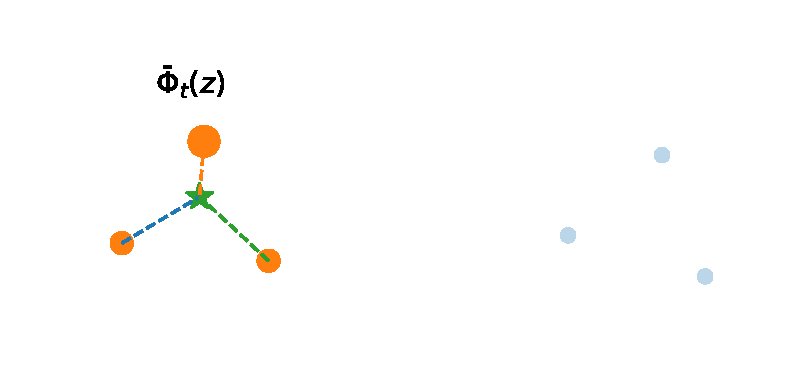
\includegraphics[width=.88\linewidth,height=1.28cm,keepaspectratio]{attachment_near.pdf}
\par\textbf{Nearby bubbles: lower dispersion}
\column{.48\textwidth}
\centering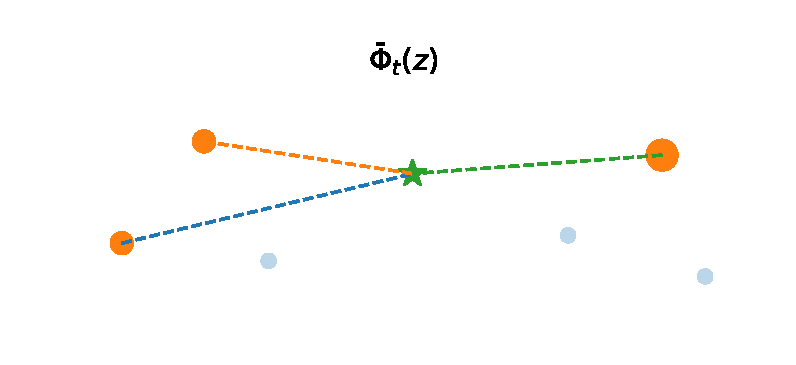
\includegraphics[width=.88\linewidth,height=1.28cm,keepaspectratio]{attachment_far.pdf}
\par\textbf{Distant bubbles: higher dispersion}
\end{columns}
\src{Schematic diffusion coordinates. Circle area: $b_j(z)$. Star: weighted mean.}
\[
\boxed{S_D(z)=\frac1{2|\TT|}\sum_{t\in\TT}\sum_{i,j}b_i(z)b_j(z)D_{t,L}^2(i,j).}
\]
\begin{columns}[T,onlytextwidth]
\column{.50\textwidth}
\head{Equivalent variance at time $t$}
\[
\begin{aligned}
\bar\Phi_t(z)&=\sum_jb_j(z)\Phi_t(B_j),\\[0.2em]
S_{D,t}(z)&=\sum_jb_j(z)\norm{\Phi_t(B_j)-\bar\Phi_t(z)}^2.
\end{aligned}
\]
\column{.46\textwidth}
\head{Frame inconsistency}
\[
S_F(z)=\tfrac12\sum_{i,j}b_i(z)b_j(z)r_F(i,j).
\]
\remarktext{Executed: $\TT=\{1,3,5\}$.}
\end{columns}
\src{A one-bubble outlier can have $S_D\approx0$; $S_B$ and $S_A$ still measure its absolute mismatch.}
\end{frame}

\def\phase{NBD MODEL}
\begin{frame}[t]{NBD: component scaling and final score}
\small
\setlength{\abovedisplayskip}{3pt}\setlength{\belowdisplayskip}{3pt}
\begin{block}{Local fit + diffusion and frame consistency}
\[
\boxed{S_{\rm NBD}(z)=\widetilde S_B(z)+\widetilde S_A(z)+\widetilde S_D(z)+\lambda_F\widetilde S_F(z).}
\]
\end{block}
\textbf{NBD only:} $\mathcal Z_{\rm cal}$ contains patches from the 721 reserved normal images:
\[
\widetilde S_q(z)=-\log\!\left[
\frac{1+\sum_{u\in\mathcal Z_{\rm cal}}\mathbf1_{\{S_q(u)\ge S_q(z)\}}}{|\mathcal Z_{\rm cal}|+1}
\right],\qquad q\in\{B,A,D,F\}.
\]
\vspace{0.02cm}
\begin{center}

\begin{tikzpicture}[box/.style={rounded corners=3pt,minimum height=.60cm,text width=3.9cm,align=center,inner sep=4pt},arr/.style={-{Latex[length=2mm]},thick,draw=teal}]
\node[box,fill=softblue] (z) {Patch features $z_p$};
\node[box,fill=softgreen,right=.40cm of z] (a) {Patch scores $A(x)$};
\node[box,fill=softorange,right=.40cm of a] (s) {Image score};
\draw[arr](z)--(a);\draw[arr](a)--(s);
\end{tikzpicture}
\end{center}
\begin{columns}[T,onlytextwidth]
\column{.43\textwidth}
\[
A(x)_p=S_{\rm NBD}(z_p).
\]
\column{.53\textwidth}
\[
S_{\rm image}(x)=\frac1{|\mathcal P_\rho(x)|}\sum_{p\in\mathcal P_\rho(x)}A(x)_p.
\]
\end{columns}
\src{$\mathcal P_\rho$: top 1\% (8 of 784 patches). $\lambda_F=1$. This is not a calibrated anomaly probability.}
\vspace{0.0cm}
\band{\footnotesize Component scaling uses the reserved subset, not the 734 threshold images.\\[.06cm]
After aggregation, NBD uses the same image-threshold rule as the baselines.}
\end{frame}

\def\phase{NBD COMPARISON}
\begin{frame}[t]{NBD versus the baseline methods}
\centering
\vspace{.03cm}
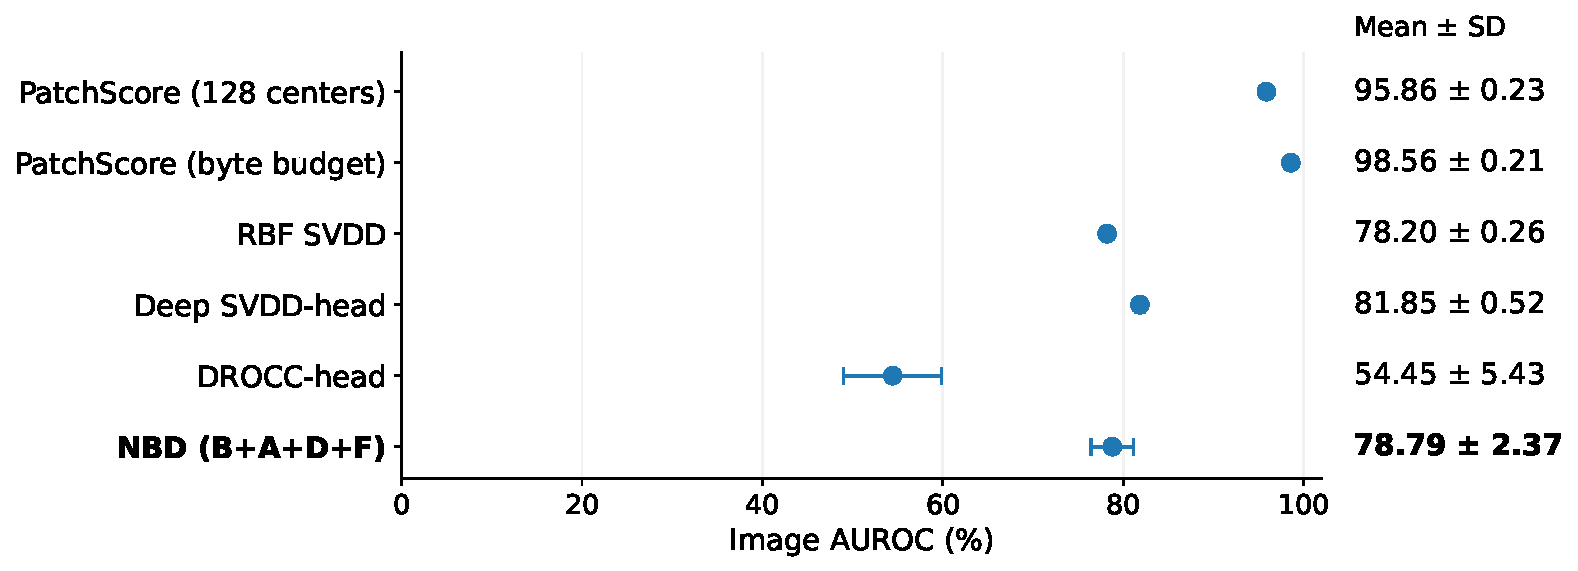
\includegraphics[width=.97\textwidth,height=3.84cm,keepaspectratio]{mvtec_nbd_comparison.pdf}
\raggedright
\remarktext{The 128-center PatchScore row is unchanged. The extra byte-budget control stores normal patches up to the NBD geometry/graph array budget; CNN and calibration state are excluded.}
\vspace{.06cm}
\band{\small NBD minus 128 centers: $-17.07\pm2.22$ pp.\\[.05cm]
NBD minus byte budget: $-19.77\pm2.29$ pp.}
\resultsrc{\texttt{summary.csv}, \texttt{paired\_deltas.csv}. Same data, seeds, CNN and top-1\% aggregation. NBD is $B+A+D+F$.}
\end{frame}

\def\phase{NBD ABLATION}
\begin{frame}[t]{Ablation: diffusion reduced AUROC in this configuration}
\small
\begin{columns}[T,onlytextwidth]
\column{.49\textwidth}
\head{Local and graph score variants}
\centering
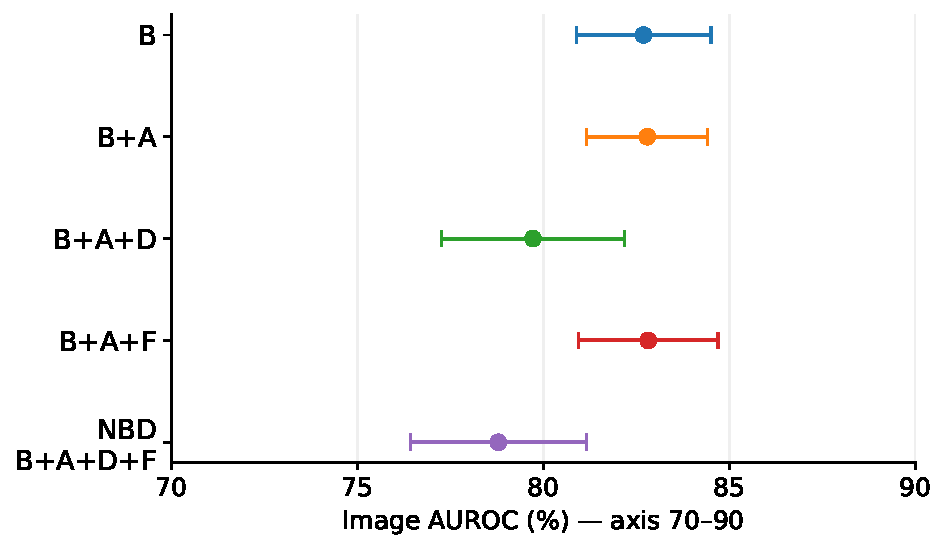
\includegraphics[width=\linewidth,height=3.22cm,keepaspectratio]{mvtec_ablations.pdf}
\raggedright
\remarktext{$B$: best bubble; $A$: soft support;\\$D$: diffusion dispersion; $F$: frame inconsistency.}
\column{.47\textwidth}
\head{Paired changes (AUROC pp)}
\renewcommand{\arraystretch}{1.65}
\begin{tabular}{lr}
\toprule
\textbf{Change}&\textbf{Mean $\pm$ SD}\\
\midrule
Add $A$ to $B$&$+0.10\pm0.20$\\
Add $D$ to $B+A$&$-3.07\pm0.92$\\
Add $F$ to $B+A$&$+0.03\pm0.61$\\
Add $D$ to $B+A+F$&$-4.03\pm0.73$\\
Add $F$ to $B+A+D$&$-0.93\pm0.33$\\
\bottomrule
\end{tabular}
\end{columns}
\vspace{.18cm}
\band{\small $B+A+F$: $82.82\pm1.88\%$.\quad Declared NBD: $78.79\pm2.37\%$.\\[.06cm]
The better ablation remains an ablation, not the final NBD result.}
\vfill
\resultsrc{\texttt{summary.csv}, handoff. Differences describe this fixed setup; they do not establish a general cause.}
\end{frame}

\def\phase{NBD COMPARISON}
\begin{frame}[t]{All 15 categories, all 10 variants}
\centering
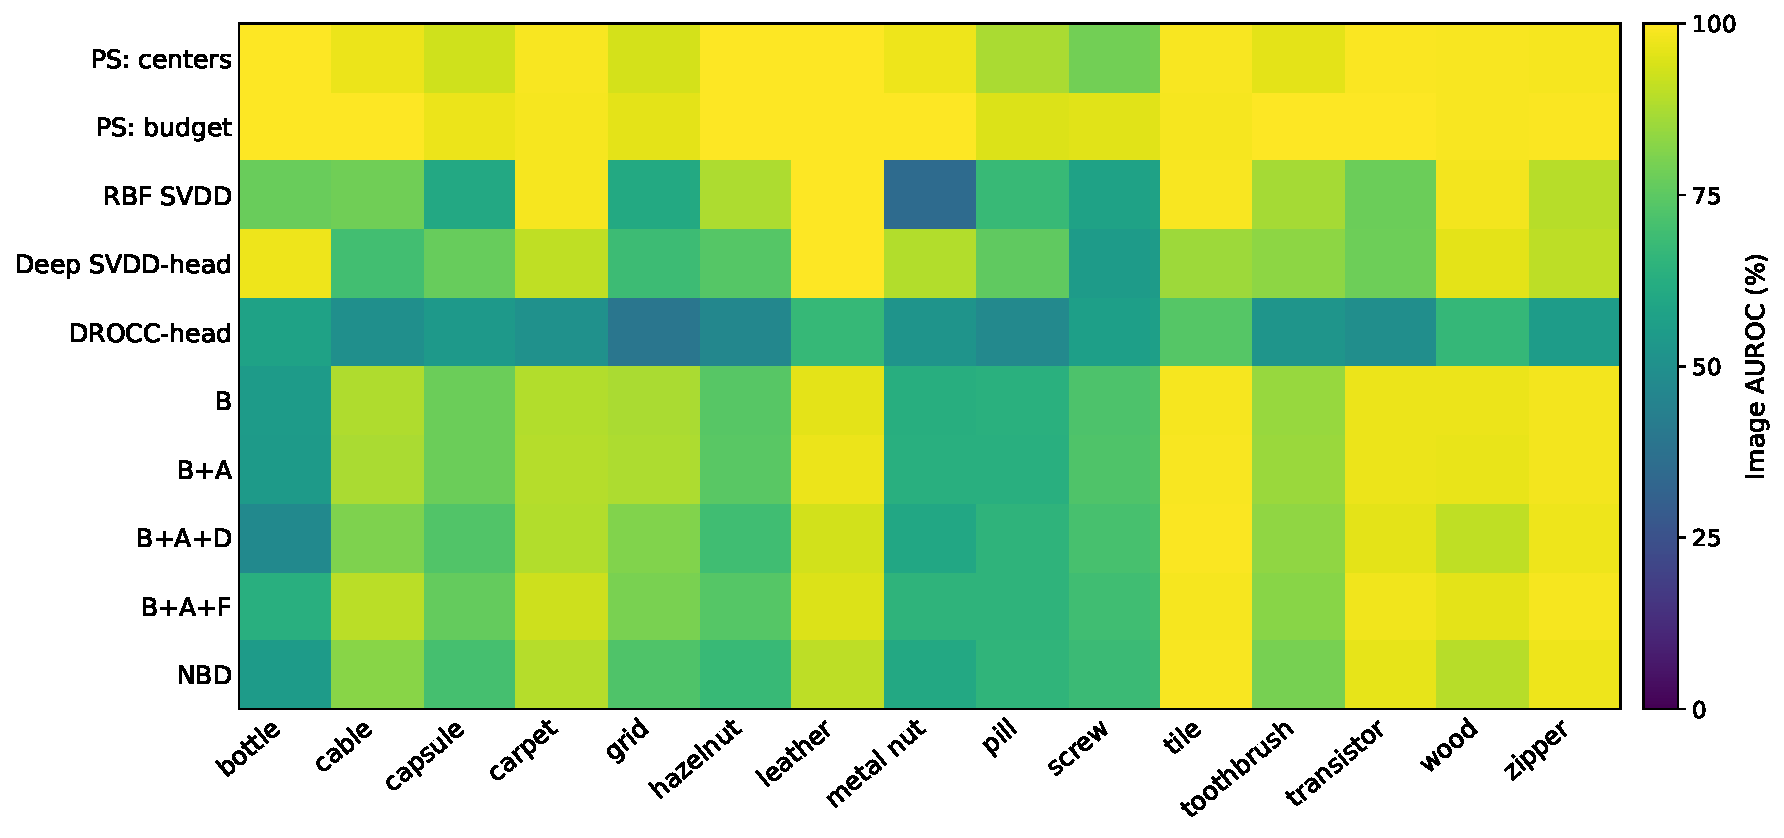
\includegraphics[width=.99\textwidth,height=4.84cm,keepaspectratio]{mvtec_categories.pdf}
\par\vspace{.05cm}
\raggedright
\band{\small NBD ranges from 54.84\% on bottle to 99.17\% on tile.\\[.07cm]
The full color scale is 0--100\%; results below 50\% remain visible.}
\resultsrc{\texttt{category\_summary.csv}. Each cell is the mean of three seeds; exact values are included in the CSV.}
\end{frame}

\def\phase{APPENDIX}
\begin{frame}[t]{Appendix: complete measured results}
\footnotesize
\vspace{.06cm}
\begin{center}
\renewcommand{\arraystretch}{1.15}\setlength{\tabcolsep}{6pt}
\begin{tabular}{lrrrr}
\toprule
\textbf{Method}&\textbf{Image AUROC (\%)}&\textbf{AP (\%)}&\textbf{FPR (\%)}&\textbf{TPR (\%)}\\
\midrule
PatchScore (128 centers) & $95.86\pm0.23$ & $98.67\pm0.05$ & 11.36 & 79.28 \\
PatchScore (byte budget) & $98.56\pm0.21$ & $99.59\pm0.06$ & 13.23 & 87.04 \\
RBF SVDD & $78.20\pm0.26$ & $90.46\pm0.17$ & 6.86 & 45.26 \\
Deep SVDD-head & $81.85\pm0.52$ & $91.58\pm0.32$ & 6.88 & 49.56 \\
DROCC-head & $54.45\pm5.43$ & $75.73\pm3.29$ & 3.51 & 8.38 \\
Bubble $B$ & $82.70\pm1.81$ & $93.19\pm0.85$ & 11.78 & 54.04 \\
Bubble $B{+}A$ & $82.80\pm1.62$ & $93.26\pm0.75$ & 11.07 & 53.80 \\
Bubble $B{+}A{+}D$ & $79.72\pm2.46$ & $91.53\pm1.29$ & 10.31 & 47.72 \\
Bubble $B{+}A{+}F$ & $82.82\pm1.88$ & $93.27\pm0.91$ & 10.89 & 53.20 \\
\textbf{NBD} $(B{+}A{+}D{+}F)$ & $78.79\pm2.37$ & $91.06\pm1.44$ & 10.81 & 47.27 \\
\bottomrule
\end{tabular}
\end{center}
\vspace{.02cm}
\remarktext{AUROC/AP: category-macro mean $\pm$ sample SD across three seeds. FPR/TPR: macro means at normal-only thresholds.}
\band{\small NBD at its normal-only threshold: FPR 10.81\%, TPR 47.27\%. No test-optimized cutoffs.}
\vfill
\resultsrc{Unmodified values from \texttt{summary.csv}; tables are generated from full-precision CSV values.}
\end{frame}

\def\phase{REFERENCES}
\begin{frame}[t]{References and benchmark files}
\small
\begin{columns}[T,onlytextwidth]
\column{.55\textwidth}
\head{Method sources}
\textbf{[1]} Tax and Duin (2004).\\
\href{https://doi.org/10.1023/B:MACH.0000008084.60811.49}{\emph{Support Vector Data Description.}}\\[.20cm]
\textbf{[2]} Ruff et al. (2018).\\
\href{https://proceedings.mlr.press/v80/ruff18a.html}{\emph{Deep One-Class Classification.}}\\[.20cm]
\textbf{[3]} Goyal et al. (2020).\\
\href{https://proceedings.mlr.press/v119/goyal20c.html}{\emph{DROCC: Deep Robust One-Class Classification.}}\\[.20cm]
\textbf{[4]} Coifman and Lafon (2006).\\
\href{https://doi.org/10.1016/j.acha.2006.04.006}{\emph{Diffusion maps.}}\\[.20cm]
\href{https://github.com/amazon-science/patchcore-inspection}{PatchCore reference implementation}\quad
\href{https://www.mvtec.com/research-teaching/datasets/mvtec-ad}{MVTec AD}
\column{.41\textwidth}
\head{Executed benchmark}
\href{https://github.com/dathuynh1108/OCC/tree/91223d63adc3289786bbdeff16d5feeb59aeb3d7}{\texttt{dathuynh1108/OCC @ 91223d6}}\\[.08cm]
\texttt{results/mvtec-full-v2/}\\
\texttt{REPORT.md}, \texttt{summary.csv}\\
\texttt{category\_summary.csv}\\
\texttt{paired\_deltas.csv}\\
\texttt{SLIDE\_UPDATE\_HANDOFF.md}\\[.16cm]
Locked settings: \texttt{configs/full.json}.\\
Backbone: WRN-50-2, ImageNet-1K V1.
\vspace{.20cm}
\head{This slide package}
\texttt{review.tex}, \texttt{assets/},\\
CSV snapshots and plotting code.\\[.12cm]
Reported audit: 450 metric rows; 51,750 image predictions. Replay: 135 groups; max error 0.0.
\end{columns}
\vfill
\resultsrc{Snapshot: 14 September 2026. No benchmark was rerun for this editorial update.}
\end{frame}

\def\phase{REPRODUCTION LINKS}
\begin{frame}[t]{GitHub sources and rerun scope}
\small
\renewcommand{\arraystretch}{1.28}
\begin{tabularx}{\textwidth}{@{}p{2.25cm}Y@{}}
\toprule
\textbf{Method}&\textbf{Clickable GitHub source}\\
\midrule
PatchCore & \href{https://github.com/amazon-science/patchcore-inspection/tree/fcaa92f124fb1ad74a7acf56726decd4b27cbcad}{\textcolor{teal}{amazon-science/patchcore-inspection}}\quad\texttt{fcaa92f}\\
SVDD & \href{https://github.com/DMJTax/dd_tools/tree/efaaf04efae1f8be78906836a5d31547b48be7af}{\textcolor{teal}{DMJTax/dd\_tools}}\quad\texttt{efaaf04}\quad(author MATLAB reference)\\
Deep SVDD & \href{https://github.com/lukasruff/Deep-SVDD/tree/e20f18c8d0ad9dc01cad09fdf311bd861351a9ad}{\textcolor{teal}{lukasruff/Deep-SVDD}}\quad\texttt{e20f18c}\quad(original paper code)\\
& \href{https://github.com/lukasruff/Deep-SVDD-PyTorch/tree/1901612d595e23675fb75c4ebb563dd0ffebc21e}{\textcolor{teal}{lukasruff/Deep-SVDD-PyTorch}}\quad\texttt{1901612}\quad(author port)\\
DROCC & \href{https://github.com/microsoft/EdgeML/tree/81025fce8ba28707eabe72e11bf3987a8d745608/examples/pytorch/DROCC}{\textcolor{teal}{microsoft/EdgeML / examples/pytorch/DROCC}}\quad\texttt{81025fc}\\
Our results & \href{https://github.com/dathuynh1108/OCC/tree/91223d63adc3289786bbdeff16d5feeb59aeb3d7/results/mvtec-full-v2}{\textcolor{teal}{dathuynh1108/OCC / results/mvtec-full-v2}}\quad\texttt{91223d6}\\
\bottomrule
\end{tabularx}
\vspace{.12cm}
\begin{columns}[T,onlytextwidth]
\column{.48\textwidth}
\head{A. Native-source reproduction}
Use each paper's data and training.\\
Keep paper/code discrepancies explicit.
\column{.48\textwidth}
\head{B. Controlled NBD rerun}
Share the author PatchCore encoder.\\
Label changed methods as adaptations.
\end{columns}
\vspace{.12cm}
\band{\footnotesize Source audit and run instructions: \texttt{handoff/CODEX\_REPRODUCE.md}.\\[.05cm]
Native-source reruns are \textbf{pending}. Existing numbers remain the measured v2 results.}
\end{frame}

\end{document}
